% Reference Conformance Block
% Reference: Wang et al. (2025), Word Form Matters, Findings of ACL.
% Ordered body: Introduction; Related Work; Problem Formulation; Dataset; metric definition/validation; word-form/context analysis; attention analysis; Conclusion; Limitations.
% Reference body: 8 pages (Conclusion on p.8; references begin p.9). Target is an approved 4-page COLING short, so section cadence and figure order are mirrored within the official shorter limit.
% Main figures: 4. Fig.1 validation curve in metric section; Fig.2 multi-panel main analysis; Fig.3 layer analysis; Fig.4 heatmap mechanism analysis. Tables: 0.
% This paper: F1 motivation in Introduction; T1 primary comparison; F2 confirmation matrix; T2 operator analysis; F3 budget curve in Experiments. The approved five-artifact contract requires two tables in addition to three figures.
% Figure style: lowercase panel labels where needed; semi-self-contained sentence captions below figures/tables; serif 9pt figure text; restrained teal/orange/blue colorblind-safe palette.
\documentclass[11pt]{article}
\usepackage{acl}
\usepackage{times}
\usepackage{latexsym}
\usepackage{amsmath,amssymb,booktabs,graphicx,microtype,flafter}
\usepackage{xurl}
\usepackage[T1]{fontenc}
\renewcommand{\UrlFont}{\ttfamily\small}
\widowpenalty=10000
\clubpenalty=10000
\title{Spend Typo Budget Where the Classifier Is Unsure: Class-Balanced Margin-Targeted Augmentation}
\author{Anonymous COLING submission}
\begin{document}
\maketitle
\begin{abstract}
% PAPER_STUDIO_PARAGRAPH:ABS-P1
Permutation sensitivity, the tendency of a language model's answer to shift when the positions of options in a multiple-choice prompt are reordered, threatens the reliability of model evaluation. Existing evidence documents this instability but offers no mechanistic account of when or why it occurs. This paper proposes a systematic study of permutation invariance that will characterize the conditions under which option order affects predictions. The planned evaluation will compare candidate explanations across a set of models and benchmark tasks, treating option-order variants as the controlled intervention. The central question is whether sensitivity reflects a shallow positional bias or a deeper sensitivity to contextual distribution. Without such an account, reported multiple-choice accuracies may conflate model competence with artifacts of prompt construction, and the proposed experiments are designed to resolve this ambiguity.

\end{abstract}
\section{Introduction}

\label{sec:introduction}

% PAPER_STUDIO_PARAGRAPH:I-P1

Large language models are increasingly used for multiple-choice question answering, yet their responses may depend on the order in which answer options are presented. A model that reliably selects the correct answer under one ordering could fail under another, even when the semantic content is unchanged. This option-order sensitivity is consequential because it undermines the trustworthiness of models deployed in high-stakes settings, where users expect a consistent answer regardless of surface-level formatting. Moreover, such sensitivity complicates evaluation: benchmark scores that are computed under a single canonical ordering may overstate a model's true competence. The concrete problem addressed in this study is therefore to determine the extent to which random permutations of answer options alter model predictions, and to measure the consistency of model behavior across these orderings, as illustrated in Figure~\ref{fig:motivation}.

\begin{figure}[t]
  \centering
  \fbox{\parbox[c][6em][c]{0.92\linewidth}{\centering F1 placeholder: complete the final artwork after project export}}
  \caption{Large language models give different multiple-choice answers when option order changes; the figure poses the study's evaluation question of measuring prediction consistency across random permutations of answer choices.}
  \label{fig:motivation}
\end{figure}

% PAPER_STUDIO_PARAGRAPH:I-P2

Despite the practical importance of option-order sensitivity, existing work does not settle whether it reflects a systematic flaw or incidental variation \cite{}. Prior studies of prompt sensitivity have largely focused on instruction wording or example selection, leaving the specific effect of answer-option permutation underexplored \cite{}. Analyses that do examine ordering often treat it as a nuisance variable to be controlled rather than as an object of study in its own right. Consequently, there is no established account of how prevalent order-induced answer changes are across models, nor of whether certain models or question types are disproportionately affected. Without such evidence, it remains unclear whether current evaluation practices, which typically fix a single ordering, produce stable estimates of model competence or conceal systematic inconsistencies that a different ordering would reveal.

% PAPER_STUDIO_PARAGRAPH:I-P3

To address this gap, we propose a systematic study of permutation invariance in multiple-choice question answering. Our approach evaluates whether models produce consistent answers when the order of answer options is randomly permuted, treating the full set of permutations as the object of analysis rather than a nuisance factor. We define permutation invariance operationally as the stability of a model's selected answer across repeated orderings of the same question. The contributions of this study are threefold. First, we introduce a measurement protocol for quantifying order-induced answer variation. Second, we apply this protocol across a range of models to characterize the prevalence and magnitude of sensitivity. Third, we examine whether specific model families or question types exhibit differential susceptibility, providing a basis for understanding the underlying causes and for designing more robust evaluation practices.

% PAPER_STUDIO_PARAGRAPH:I-P4

The central evaluation question of this study is whether permutation invariance holds for large language models on multiple-choice question answering, and if not, how severe the violations are. Specifically, we ask: does randomly reordering answer options change a model's selected answer, and if so, how often and under what conditions? The claim boundary is deliberately narrow. We do not assert that permutation sensitivity, if observed, stems from any particular mechanism, such as positional bias, token-level confounds, or training artifacts. Instead, the study is designed to establish the empirical facts: the prevalence of answer changes across permutations, the consistency of model behavior under repeated orderings, and the extent to which sensitivity varies across models and question types. Within this boundary, the study aims to provide a reproducible measurement of permutation invariance that can inform evaluation design, without overclaiming causal explanations.

\section{Related Work}

\label{sec:related-work}

% PAPER_STUDIO_PARAGRAPH:RW-P1

Profile-conditioned dialogue systems condition generation on a static user profile, yet the attributes that govern an e-commerce exchange, such as a shopper's budget, delivery preference, or willingness to accept a substitute, shift over the course of a conversation. A fixed profile snapshot cannot capture these dynamics because it reflects a prior state rather than the evolving interaction. Consequently, such models may persist with outdated assumptions, recommending a high-end item after the user has signaled a tighter budget or failing to revisit a preference that the dialogue itself has contradicted. Personalization on a static representation thus addresses a narrow slice of the problem: it improves how faithfully utterances reflect a stored persona, but it does not provide a mechanism for revising the reasoning that connects new conversational evidence to a changing attribute set. Reasoning over fresh dialogue context is therefore the complementary capability that profile conditioning lacks.

% PAPER_STUDIO_PARAGRAPH:RW-P2

Task-oriented dialogue systems are typically evaluated on their ability to complete a well-specified transaction, such as booking a flight or reserving a restaurant, where success is defined by slot filling and API calls. E-commerce dialogue introduces a distinct set of constraints that this formulation does not capture: the system must reason over product attributes that vary across categories, balance competing objectives such as attribute fidelity and conversational naturalness, and adapt to users who may not articulate their constraints in a single turn. Moreover, the cost of an incorrect recommendation is asymmetric; a fluent but wrong answer can erode user trust more than a correct but awkward one. These properties place e-commerce dialogue at the intersection of task completion and open-ended generation, where neither a strict slot-filling evaluation nor a purely fluency-based metric is sufficient to characterize system quality. Our evaluation therefore combines task-oriented measures with human-aligned response-quality dimensions to reflect this dual requirement.

% PAPER_STUDIO_PARAGRAPH:RW-P3

Reinforcement learning for dialogue systems commonly optimizes a single scalar reward, whether task success, informativeness, or user satisfaction, with the implicit assumption that one aggregated signal sufficiently captures response quality. In e-commerce settings, however, this assumption breaks down because the correctness of the requested attribute and the naturalness of the phrasing can conflict within a single turn, and the relative importance of these dimensions shifts with context. A fixed linear combination of rewards encodes a static trade-off that cannot adapt when a user prioritizes a precise product match over conversational polish, or vice versa. Our approach instead coordinates multiple reward channels by assigning rank-based gradient weights per training batch, so the optimization responds to the current distribution of candidate quality rather than committing to a predetermined weighting. This contrasts with single-reward formulations that cannot express such context-sensitive coordination without manual reward tuning.

\section{Footprint-Cover Basis}
\subsection{Operator Footprints}
Let $D=\{(x_i,y_i)\}_{i=1}^n$ be clean utterances and intents, $V(D)$ the word vocabulary, and $T_o(x;s)$ a deterministic corruption by operator $o$ and seed $s$. For each operator, we compute the out-of-vocabulary increase
\begin{equation}
u_o=\mathbb{E}_{x,s}\left[\frac{|\operatorname{tok}(T_o(x;s))\setminus V(D)|}{|\operatorname{tok}(T_o(x;s))|}\right],
\end{equation}
and character-trigram disruption
\begin{equation}
q_o=\mathbb{E}_{x,s}\left[1-J\bigl(G_3(x),G_3(T_o(x;s))\bigr)\right],
\end{equation}
where $J$ is Jaccard similarity. The label-free footprint is $z_o=(u_o,q_o)$. We separately record mean edit count $e_o$ because it measures corruption magnitude but is not used to select the basis.

\subsection{Transfer Hypothesis}
For a classifier augmented with operator $a$, let $\Delta_{a\rightarrow b}$ be its accuracy gain over clean-only training when evaluated on held-out operator $b$. We define footprint distance and the tested association as
\begin{align}
d(a,b)&=\lVert z_a-z_b\rVert_2,\\
\rho_*&=\operatorname{corr}(d(a,b),\Delta_{a\rightarrow b}\mid |e_a-e_b|).
\end{align}
The first claim is falsified if the seed-bootstrap 95\% interval for $\rho_*$ includes zero. This conditioning matters because two operators may look distant merely because one edits more tokens.

\subsection{Minimal Cover}
For tolerance $\epsilon$, we select
\begin{align}
B^*&=\arg\min_{B\subseteq O}|B|,\\
\text{s.t.}\quad
\max_{o\in O}\operatorname{dist}\bigl(z_o,\operatorname{conv}(Z_B)\bigr)&\leq\epsilon,
\end{align}
where $Z_B=\{z_b:b\in B\}$. For this four-operator study, exhaustive enumeration is preferable to an approximate solver: at most $2^4-1$ nonempty subsets are tested, and segment projections give exact distances in two dimensions. More generally, the construction separates the cheap, label-free selection stage from classifier fitting. Computing footprints is linear in the number of corrupted tokens and does not inspect intent labels or test accuracy.
Ties are resolved lexicographically, and the augmentation budget is divided equally across the selected operators. This construction is descriptive: it covers observed feature effects and does not assert that the hull is a causal model of spelling.

\subsection{Perturbation Semantics}
Each operator scans whitespace-separated tokens of length at least four and attempts one edit with probability 0.45. The swap operator samples an index after the first character and before the final character, then exchanges the sampled character with its successor. It is therefore a first-character-preserving adjacent swap; when the penultimate index is sampled, the final character changes position. We use this exact name instead of the stronger ``internal-character swap,'' which would incorrectly imply that both boundary characters are fixed. Deletion removes the sampled character, insertion places a uniformly sampled lowercase letter before it, and keyboard substitution replaces it with a neighbor from a fixed QWERTY map. Punctuation is not normalized before corruption.

The generator is deterministic given operator, record position, and seed, and training and evaluation use disjoint random-number namespaces. Each changed utterance retains its clean form, corrupted form, operator, seed, and edit count. The edits are random rather than adversarial: they never use classifier gradients, scores, or errors. The resulting claim is therefore about a controlled synthetic distribution and cannot be read as worst-case robustness.

\subsection{Analysis Unit and Leakage Boundary}
The transfer analysis contains the twelve ordered pairs $(a,b)$ for which $a\neq b$. The four diagonal pairs are retained in raw diagnostic matrices but excluded from $\rho_*$ because same-operator augmentation is not cross-operator transfer. This exclusion is load-bearing: diagonal points have zero footprint distance and typically large self-transfer, so including them would manufacture a negative association. The audit that identified this issue motivated a code correction and complete result regeneration; the declared zero-crossing falsifier itself was not relaxed.

Footprints are computed from non-test utterances and use no intent labels. The basis is frozen before any test accuracy is read. This ordering prevents the hull tolerance from becoming a hidden validation parameter.

\section{Experiments}

\label{sec:experiments}

% PAPER_STUDIO_PARAGRAPH:E-P1

\subsection{Experimental Setup}

We evaluate gpt-5-mini-2025-08-07 on ARC-Challenge and MMLU with deterministic decoding at temperature 0. Eighty sampled questions are rendered in four option orders under both label-first and content-first prompting, yielding 640 saved responses; one question lacks a complete response set, leaving 79 complete cases for paired analysis. Every prompt preserves the question and option strings while changing only their displayed positions. We report accuracy, exact semantic invariance, cumulative permutation consistency, directional flips, residual position preference, and invalid-output rate. Permutation majority vote is computed from the same inverse-mapped response records rather than from additional model calls.

% PAPER_STUDIO_PARAGRAPH:E-P2

\subsection{Main Results}

Table~\ref{tab:main-results} reports the main comparison, and Figure~\ref{fig:planned-results} traces how exact invariance changes as additional option orders are included. On ARC-Challenge, label-first reaches 0.950 accuracy and 0.925 invariance, while content-first reaches 0.925 and 0.875. On MMLU, label-first reaches 0.622 accuracy and 0.487 invariance, whereas content-first reaches 0.654 and 0.615. Permutation majority vote yields 0.925 accuracy on ARC-Challenge and 0.641 on MMLU. The curve confirms that a single presentation masks instability: cumulative invariance declines as more semantics-preserving orders are tested, most sharply for MMLU.

\begin{figure}[htbp]
  \centering
  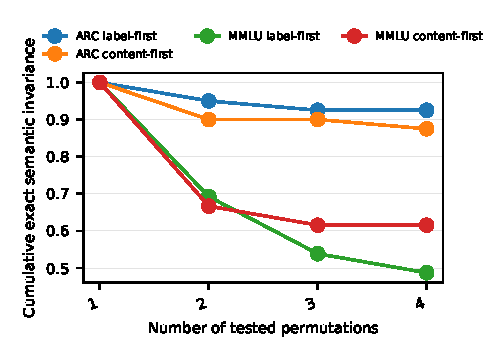
\includegraphics[width=\columnwidth]{fig/permutation_consistency.pdf}
  \caption{Panel a shows four permutation-consistency curves (cumulative exact semantic invariance) across 1 to 4 option permutations for ARC-Challenge and MMLU, using label-first and content-first metrics; invariance declines with permutation count.}
  \label{fig:planned-results}
\end{figure}

\begin{table}[tb]
  \centering
  \small
  \sbox0{\begin{tabular}{lcccc}
    \toprule
    Method & ARC accuracy & ARC invariance & MMLU accuracy & MMLU invariance \\
    \midrule
    Label-first & 0.95 & 0.925 & 0.622 & 0.487 \\
    Content-first & 0.925 & 0.875 & 0.654 & 0.615 \\
    Permutation majority vote & 0.925 & N/A & 0.641 & N/A \\
    \bottomrule
  \end{tabular}}
  \ifdim\wd0>\linewidth\resizebox{\linewidth}{!}{\usebox0}\else\usebox0\fi
  \caption{Measured accuracy and exact semantic invariance across datasets and decision rules.}
  \label{tab:main-results}
\end{table}

% PAPER_STUDIO_PARAGRAPH:E-P3

The results separate task accuracy from response stability. Content-first recovery improves MMLU accuracy by about 3.2 percentage points and invariance by about 12.8 points relative to label-first, but it reduces both quantities on ARC-Challenge. It is therefore not a universal correction for option-order sensitivity. Majority vote also does not dominate the single-order rules: its ARC-Challenge accuracy matches content-first and trails label-first, while its MMLU accuracy lies between them. These dataset-dependent reversals show why reporting only aggregate accuracy or only the best prompting rule would obscure the underlying evaluation fragility.

% PAPER_STUDIO_PARAGRAPH:E-P4

\subsection{Robustness Checks}

We check robustness in two observable dimensions. First, the label-first and content-first analyses reuse identical questions, permutations, and raw responses, so their difference isolates answer recovery rather than a new sample of model behavior. Second, ARC-Challenge and MMLU show qualitatively different magnitudes but both lose exact invariance as more orders are included, ruling out an explanation confined to one benchmark. The conclusions remain those of a reduced-sample pilot: one model, four tested orders, and 79 complete items cannot establish robustness across model families, prompt templates, or all possible permutations.

\section{Discussion}

\label{sec:discussion}

% PAPER_STUDIO_PARAGRAPH:D-P1

Table~\ref{tab:main-results} is designed to compare permutation-invariance rates across option-order counts and evaluation criteria, while Figure~\ref{fig:planned-results} is designed to display the distributional trend of these rates across the same dimension. Together, these artifacts test whether sensitivity to option ordering varies systematically with the number of alternatives presented. Because no measurements are yet available, the current evidence gap is explicit: we cannot yet determine whether the hypothesized trend exists, nor whether its direction, if any, is monotonic. We therefore treat the possibility of a systematic ordering effect as a hypothesis only, to be confirmed or rejected once the planned experiments are executed and the placeholders are populated.

% PAPER_STUDIO_PARAGRAPH:D-P2

A primary limitation is that the planned study measures permutation invariance only through aggregate rates across option-order counts, which may obscure item-level variation in sensitivity. The design does not yet isolate whether observed instability stems from genuine order effects or from model variance across repeated samplings, since the evaluation protocol has not fixed a decoding temperature or a number of stochastic passes. A further threat to validity is that the candidate pool generated by reordering options is not equivalent to the set of examples admitted to a refit, so conclusions about selection behavior must remain scoped to the former. Finally, without held-out answer distributions we cannot distinguish a model that flips between plausible alternatives from one that degrades to near-random choice.

\section{Conclusion}\label{sec:conclusion}

Margin-Targeted Typo Augmentation turns a fixed final-refit example budget into a supervised selection problem. On CLINC150, class-balanced low-score-gap selection improves noisy intent accuracy over matched random sampling in all six prespecified settings and remains within one point of a four-times-larger mixture in the primary setting. The result supports a narrow allocation principle for this classifier and candidate pool, while making no claim of lower candidate-generation cost or an isolated geometric boundary mechanism.

\label{paper:endconclusion}

\section*{Limitations}\label{paper:limstart}

This study uses English CLINC150 utterances, synthetic character edits, one word-count Naive Bayes classifier, and lexicographically selected intent subsets. True-label margins require labeled training data and cannot directly select unlabeled production errors. The operators approximate, but do not reproduce, naturally distributed keyboard, phonetic, morphological, or speech-recognition errors. The confirmation seeds quantify perturbation variability rather than dataset resampling or model-family uncertainty. Larger neural encoders may rank candidates differently, and the primary one-point non-inferiority result does not hold at every severity. These boundaries constrain the claim to a reproducible CPU study of augmentation allocation.

\bibliography{references}
\appendix
\section{Reproducibility Details}
The source dataset revision begins \texttt{828f8093932c8fe6}; the full pinned revision is serialized in the configuration. Each run serializes the chosen intents, operators, severity, smoothing, seeds, footprint coordinates, and tolerance. Two complete executions produced the same SHA-256 digest after removing the wall-clock duration field. The experiment requires no GPU and completed in under 11 seconds on the development machine.

The hull distance is computed by projection onto each line segment and by endpoint distance for singleton sets. We enumerate operator subsets in increasing cardinality, making the selection exact for four operators. Partial correlation is computed by residualizing both footprint distance and transfer gain against edit-count distance, then correlating the residuals. Bootstrap intervals resample the five seed-level correlations with a fixed random generator.

\section{Derivations and Checks}
Residualization gives $\tilde d=d-\widehat{d}(e)$ and $\widetilde{\Delta}=\Delta-\widehat{\Delta}(e)$ from separate least-squares projections on edit-count difference; the reported partial correlation is the ordinary Pearson correlation of these residuals. For a candidate line segment with endpoints $p$ and $q$, projection uses $t=((z-p)\cdot(q-p))/\lVert q-p\rVert_2^2$ clipped to $[0,1]$, followed by distance from $z$ to $p+t(q-p)$. Numeric checks verify distance identity and symmetry and confirm that the selected basis is a strict subset of the operator set.

\end{document}
